\documentclass[12pt]{article}

% =========================
% Page layout
% =========================
\usepackage[a4paper,margin=1in]{geometry}
\usepackage{setspace}
\onehalfspacing
\usepackage{indentfirst}
% =========================
% Fonts and encoding
% =========================
\usepackage[T1]{fontenc}
\usepackage[utf8]{inputenc}
\usepackage{lmodern}

% =========================
% Math, tables, figures
% =========================
\usepackage{amsmath, amssymb, amsthm}
\usepackage{booktabs}
\usepackage{threeparttable}
\usepackage{graphicx}
\usepackage{subcaption}
\usepackage{float}
\usepackage{makecell}
\usepackage{siunitx}
\usepackage{tabularx}
\usepackage{array}
% =========================
% References and hyperlinks
% =========================
\usepackage[round,authoryear]{natbib}
\usepackage[colorlinks=true,
            linkcolor=blue,
            citecolor=blue,
            urlcolor=blue]{hyperref}

% =========================
% Header and footer
% =========================
\usepackage{fancyhdr}
\pagestyle{fancy}
\fancyhf{}           
\cfoot{\thepage}      
\renewcommand{\headrulewidth}{0pt} 

% =========================
% Theorem-like environments
% =========================
\newtheorem{hypothesis}{Hypothesis}
\newtheorem{proposition}{Proposition}

% =========================
% Title information
% =========================
\title{\textbf{Modeling Profit Give-Back Risk in Algorithmic Trading via LSTM-Based Exit Decision Systems}}

\author{
First Author\thanks{
First Author: Department of Finance, XXX University.
Email: \href{mailto:first.author@email.com}{first.author@email.com}.
}
\and
Second Author\thanks{
Second Author: School of Economics, XXX University.
Email: \href{mailto:second.author@email.com}{second.author@email.com}.
}
}

\date{
This Draft: \today
}

\begin{document}

% =========================
% Title page
% =========================
\maketitle

\begin{abstract}
\noindent
This paper studies ...
We examine ...
Using ... data from ... to ..., we find that ...
The results suggest that ...
This paper contributes to the literature by ...

\vspace{0.5em}
\noindent
\textbf{Keywords:} Stablecoins; Treasury Yields; Monetary Policy Transmission; Local Projections; Financial Markets.

\vspace{0.5em}
\noindent
\textbf{JEL Classification:} E43; E44; E52; G12; G15.
\end{abstract}

\vspace{1em}

\noindent
\textbf{Acknowledgments:}
We thank ... for helpful comments and suggestions. All errors are our own.

\newpage

% =========================
% Main text
% =========================
\section{Introduction}\label{sec:introduction}

In quantitative trading, trend-following strategies have been widely adopted because of their 
structural simplicity and robustness across markets. Among them, crossover strategies based on 
moving averages (MA) or weighted moving averages (WMA) represent one of the most typical 
implementation paradigms. Such methods usually rely on moving-average crossover signals to open 
positions and reverse positions, and have shown a certain degree of effectiveness in capturing 
medium- to long-term price trends. However, although entry rules have been extensively studied 
and have become relatively mature, the optimization of exit timing remains one of the key 
factors limiting strategy performance.

Traditional trend-following strategies commonly adopt a “close on reverse signal” mechanism, 
under which a position is exited only when a trend reversal occurs and an opposite crossover 
signal is triggered. This mechanism is inherently subject to substantial lag. While it helps 
capture a complete trend interval, in the later stage of a trend or during range-bound markets, 
accumulated unrealized profits often cannot be locked in in a timely manner, leading to a 
drawdown of unrealized profits. To address this issue, existing methods typically rely on fixed 
take-profit/stop-loss rules or trailing stops. However, these methods depend on empirically 
chosen parameters, are difficult to adapt to dynamic market conditions, and lack a data-driven 
decision-making capability for determining whether a position should be exited early.

To systematically characterize this problem, this paper first conducts an empirical analysis 
of the trading paths of trend-following strategies in the cryptocurrency market and identifies 
a salient empirical fact that has not been sufficiently discussed: the vast majority of trades 
once achieved positive unrealized returns during the holding period, but only a small proportion 
eventually closed with positive returns. Specifically, in the dataset examined in this study, 
around 90\% of trades were in profit at some point, whereas only about 30\% ended as profitable 
trades. This finding suggests that the main bottleneck of trend-following strategies is not the 
absence of profit opportunities, but the lack of an effective mechanism for profit locking and 
risk control.

Based on the above observation, this paper formalizes the phenomenon as unrealized profit 
drawdown risk and models it as a sequential decision-making problem: during the holding period, 
how can one determine, based on the current market state and position-related characteristics, 
whether continued holding will lead to a significant future drawdown in returns, and thereby 
decide whether the position should be exited early? Unlike traditional approaches that focus 
on price prediction or trend identification, this paper emphasizes the dynamic evolution of 
the profit path and its associated risk structure.

To this end, this paper proposes an early-closing decision framework based on Long Short-Term 
Memory (LSTM). The proposed method formulates the exit problem as a sequence classification 
task. By taking as input time-series data containing both market features and position-context 
information, the model learns the probability of executing a closing operation at the current 
time. Furthermore, this paper designs a value-based labeling function grounded in the 
trade-off between future returns and drawdowns, enabling the model to directly learn the 
decision boundary of whether ``continued holding is preferable to early exit.'' From a system 
perspective, the model can be regarded as a data-driven decision layer embedded on top of a 
traditional trend-following strategy, with the aim of improving the quality of exit decisions. 
In the empirical analysis, this paper conducts backtesting based on the cryptocurrency market. 
The results show that, while overall returns remain broadly stable, the proposed method 
significantly improves the strategy's win rate and Sharpe ratio, and effectively reduces the 
maximum drawdown.

% The remainder of the paper is organized as follows.Section~\ref{sec:literature} reviews the 
% related literature in this field.Section~\ref{sec:analysisGiveBack} describes the empirical analysis of the
% profit giving-back phenomenon.Section~\ref{sec:methodology} presents the strategy and how it 
% works.Section~\ref{sec:results} reports the experimental design.Section~\ref{sec:mechanism} 
% reports and discusses our results.Section~\ref{sec:conclusion} extends our methodology to 
% different assets,adds transaction costs and adjust the parameters to check the robustness of 
% our results.Section~\ref{sec:conclusion} concludes the paper and discusses directions for 
% future research.

\section{Literature Review}\label{sec:literature}

The central issue in quantitative trading research is how to identify exploitable price 
regularities from historical market information and transform them into trading strategies that 
can be implemented on a sustainable basis. Around this issue, the related literature has 
broadly evolved from traditional technical-analysis rules to machine-learning-based prediction, 
and further to reinforcement-learning-based dynamic decision making. Early studies mainly 
relied on trend-following rules such as moving averages, moving-average crossovers, and 
momentum, generating buy and sell signals directly from price series. Subsequently, 
machine learning methods began to be widely used for price-direction prediction, return 
prediction, and trading-signal identification. In recent years, reinforcement learning has 
further framed trading as a sequential decision-making problem, making take-profit, stop-loss, 
and dynamic exit optimization increasingly important research topics. Overall, the existing 
literature has accumulated relatively rich findings on how to identify opportunities and how to 
predict prices, but there remain clear limitations in how to optimize exit timing and how to 
reduce the drawdown of profits.

\subsection{Trend-following Strategies}

Trend-following strategies are among the most classical research directions in quantitative 
trading. Their basic idea is to exploit price inertia by using technical indicators to identify 
trends and trade in the direction of those trends. Moving-average-based methods are the most 
representative strategies in this field, including the simple moving average (SMA), weighted 
moving average (WMA), exponential moving average (EMA), and short--long moving-average 
crossover rules. \citet{Hunter1986} provided an early systematic discussion of the exponentially 
weighted moving average, emphasizing the importance of recent information in time-series 
analysis; \citet{Hansun2013} further discussed possible improvements to moving-average methods 
on this basis, showing that traditional moving-average tools themselves have continued to 
evolve.

As research developed, scholars were no longer satisfied with treating moving-average rules as 
purely empirical trading tools, and began to examine their effectiveness from both theoretical 
and empirical perspectives. \citet{ChiarellaHeHommes2006} analyzed the mechanism of 
moving-average rules from the perspective of a dynamic market model, pointing out that the 
length of the moving-average window and feedback from trading behavior can significantly 
affect price dynamics. \citet{EllisParbery2005} compared adaptive moving-average and simple 
moving-average strategies, showing that dynamic adjustment of moving-average parameters can 
help improve strategic adaptability. \citet{MarshallNguyenVisaltanachoti2017} further compared 
time-series momentum with moving-average rules, noting that although both are based on the 
idea of trend continuation, they differ in signal construction and sources of returns.

Overall, the evolution of trend-following strategies has moved from single rules with fixed 
windows and fixed thresholds toward parameter adaptation and more diversified rule structures. 
For this reason, traditional technical analysis has not lost its value with the development of 
machine learning. Instead, it has become an important source of features for subsequent 
intelligent trading models. The study by \citet{AyalaEtAl2021}, for example, shows that 
technical-analysis strategies are increasingly being re-coded, optimized, and integrated 
by machine learning methods, thereby enabling a methodological transition from rule-driven to 
data-driven approaches.

\subsection{Machine Learning in Trading}

After machine learning entered the field of quantitative trading, the research paradigm changed 
markedly. Unlike traditional technical analysis, which relies on rules predefined by researchers, 
machine learning emphasizes automatically learning the mapping between historical data, price 
changes, and trading outcomes. Early representative work such as \citet{TrippiDeSieno1992} had 
already attempted to use neural networks for stock-index futures trading, indicating that 
researchers had long recognized the possibility that complex nonlinear relationships behind 
price movements could be captured by models. Subsequently, \citet{DempsterJones2001} used 
genetic programming to improve trading rules, while \citet{DempsterLeemans2006} applied 
reinforcement learning to automated foreign-exchange trading, both reflecting the gradual 
shift of quantitative trading research from manual rule design toward intelligent decision
making.

In terms of method types, the application of supervised learning in quantitative trading can 
mainly be divided into classification and regression. Classification methods are usually used 
to predict price directions, trend reversals, or buy and sell signals. For example, studies such 
as \citet{ShenJiangZhang2012} and \citet{GerleinEtAl2016} focus on directional prediction and 
trading classification in stock markets. Regression methods, by contrast, are more often used 
to predict future price levels and returns, with the emphasis placed on improving numerical 
forecasting accuracy and supporting subsequent trade execution. \citet{ZhongEnke2019} predicted 
the daily return direction of the stock market using hybrid machine learning algorithms, 
demonstrating the practical value of classification models in generating trading signals. 
\citet{AdegboyeKampouridis2021} discussed the applicability of both classification and 
regression models to the prediction of directional-change trends and directional reversals in 
the foreign-exchange market, indicating that the two are not substitutes for one another in 
quantitative trading, but instead serve different objectives.

In this process of development, the LSTM model became an important milestone in quantitative 
finance research. Since financial time series typically exhibit nonlinearity, time variation, 
and long-term dependence, traditional machine learning models often face insufficient memory 
capacity when dealing with such data. Through its gating mechanism, LSTM can better retain 
long-term information, and thus quickly became a core tool for price prediction and 
trading-signal modeling. \citet{NelsonPereiraDeOliveira2017} used LSTM to predict stock price 
directions, providing an early demonstration of the model's applicability to financial sequence 
forecasting. \citet{FischerKrauss2018} further demonstrated the significant advantages of LSTM 
in financial market direction prediction. Later, \citet{BorovkovaTsiamas2019} extended LSTM to 
high-frequency stock classification and improved the model's robustness in non-stationary 
markets through an ensemble approach. Studies such as \citet{MehtabSenDutta2020} and 
\citet{GhoshEtAl2022} further show that LSTM, as well as hybrid architectures combining LSTM 
with CNNs, random forests, XGBoost, and other models, has become an important technical route 
in quantitative trading research.

More recently, the focus of machine learning research has no longer been confined to whether 
prediction is accurate, but has gradually shifted toward whether models genuinely improve 
trading performance. In a study of the cryptocurrency market, \citet{SebastiaoGodinho2021} 
emphasized that model performance differs significantly across market states, suggesting that 
in-sample accuracy cannot be directly translated into stable trading profits. 
\citet{HanKimEnke2023}, from the perspective of label design, linked price prediction more 
closely with trading-system construction. This indicates that machine learning research in 
quantitative trading has gradually moved from pure price prediction toward a profit-oriented 
and strategy-oriented practical framework.

\subsection{Exit Strategy Optimization}

Compared with the large body of research focusing on the identification of entry signals, the 
optimal exit strategy concerns the question of when to close a position, which has a more 
direct impact on the realization of trading profits. Exit decisions not only determine the 
final profit or loss of individual trades, but also relate to profit protection and the control 
of risk exposure, and are therefore of great importance in actual trading.

Early studies on exit problems mainly focused on fixed stop-loss and fixed take-profit rules. 
\citet{LeungLi2015} introduced transaction costs and stop-loss exit constraints into a 
mean-reversion trading framework, pointing out that the setting of exit boundaries directly 
affects strategy optimality. \citet{LoRemorov2017} further analyzed the effectiveness of 
stop-loss strategies in the presence of serial correlation, regime switching, and transaction 
costs, showing that stop-loss rules do not unconditionally improve the risk--return profile in 
all environments, but depend heavily on market states and parameter settings. 
\citet{VezerisKyrgosSchinas2018} compared the performance of multiple take-profit and stop-loss 
strategies in combination with an MACD system, finding that volatility-based dynamic 
thresholds have stronger adaptability than fixed thresholds.

On this basis, research on trailing stop-loss rules began to attract attention. The core 
function of a trailing stop is not merely to limit losses; more importantly, as prices move in 
a favorable direction, the exit threshold is raised accordingly, thereby locking in part of the 
paper profit and reducing the drawdown of profits. \citet{GlynnIglehart1995} provided an early 
theoretical discussion of the trading implications of trailing stops. \citet{DaiEtAl2021} 
showed from a risk-control perspective that trailing stop-loss rules can effectively reduce 
total risk and downside risk in declining markets. \citet{LeungZhang2021} further formulated 
trailing stops as an optimal stopping problem with path-dependent constraints, promoting the 
development of exit-decision research from empirical rules toward theoretical optimization 
models.

In recent years, reinforcement learning has provided new methodological tools for the study of 
optimal exits. Unlike supervised learning, which focuses on predicting future prices, 
reinforcement learning is better suited to handling the sequential decision problem of what 
action should be taken under a given market state, and is therefore naturally applicable to 
position management and exit-timing optimization. \citet{KimKim2019} applied deep reinforcement 
learning to the optimization of trading boundaries and stop-loss boundaries in pairs trading. 
\citet{TsantekidisEtAl2020} proposed a deep reinforcement learning framework based on price 
trailing, directly improving exit quality during the trading process through a modified reward 
function. The DeepTrader model of \citet{WangEtAl2021} and the review by \citet{SunWangAn2023} 
further show that reinforcement learning has become an important frontier in quantitative 
trading, especially in dynamic asset allocation and trade execution.

However, judging from the distribution of existing studies, reinforcement learning is still more 
often used for overall trading decisions, asset allocation, and direction selection, rather than 
for the systematic optimization of the exit timing of individual trades. \citet{HwangEtAl2023} 
pointed out that stop-loss mechanisms in actual trading often change the effectiveness of the 
original buy and sell signals, indicating that correct prediction does not necessarily imply 
profitable trading, and that exit rules play a decisive role in this process. Although 
\citet{SivriEtAl2023} and \citet{Shawky2023} have begun to directly use machine learning to 
determine stop-loss and take-profit levels, the number of such studies remains relatively 
limited, suggesting that optimal exit remains an important topic in quantitative trading 
research that has not yet been sufficiently developed.

Existing studies have produced relatively rich findings in trend identification, price 
prediction, and the construction of automated trading systems, but there remain several clear 
shortcomings in exit optimization, especially in the control of profit drawdowns.

First, although traditional trend-following strategies are intuitive and interpretable, they are 
highly sensitive to parameter settings, sample periods, and market environments. Once the 
moving-average window and trend-identification rules are set inappropriately, strategy 
performance may fluctuate significantly. This suggests that traditional rules often lack 
robustness in markets and find it difficult to adapt continuously to different volatility 
states and structural changes.

Second, the overall amount of research on optimal exits remains limited, and its internal 
development is uneven. Existing studies pay more attention to when to buy and whether prices 
will rise, while the questions of when to sell and how to reduce the drawdown of profits remain 
insufficiently discussed. In particular, compared with research on stop-loss rules, the 
literature on take-profit rules, trailing take-profit mechanisms, and the joint optimization of 
take-profit and stop-loss rules is more limited.

Third, most existing studies treat entry, holding, and exit separately, and have not yet formed 
a unified optimization framework running through trend identification, signal generation, and 
dynamic exit. In real trading, the final performance of a trade does not depend only on whether 
the entry point is accurate, but also heavily on risk management during the holding period and 
the method of exit. If the exit mechanism is poorly designed, even strong predictive ability 
may be eroded by profit drawdowns, frequent stop-loss triggers, or transaction costs. Therefore, 
future research needs to integrate prediction models and exit decisions more closely, and incorporate profit protection, drawdown control, and risk-adjusted returns into a unified objective function.

In summary, the existing literature has provided a relatively solid research foundation for 
trend following, machine-learning-based prediction, and reinforcement-learning-based trading, 
but research on optimal exit, especially the control of profit drawdowns, remains clearly 
insufficient. For this reason, starting from dynamic take-profit and trailing exit mechanisms, 
and combining them with machine learning methods to build a unified decision-making framework 
that is closer to real trading environments, has not only clear theoretical significance but 
also strong practical value.


% To print the bibliography in a standalone document, add:
% \bibliographystyle{plainnat}
% \bibliography{references}


\section{Empirical Analysis of Profit Give-Back}\label{sec:analysisGiveBack}

\subsection{Definition of Key Indicators}

To systematically characterize the profit evolution path of the trend-following strategy during the holding period and its drawdown features, this paper defines the following key indicators:

\textbf{Maximum Favorable Excursion (MFE)}:MFE refers to the highest unrealized profit level 
reached by a trade over its entire holding period, and is used to measure the maximum potential 
profit that the trade once achieved along its path. It is defined as follows:

\begin{equation}
    MFE = \max_{t \in [t_{entry}, t_{exit}]} PnL(t)
\end{equation}

where $PnL(t)$ denotes the unrealized profit or loss of the trade at time $t$.

MFE reflects the ``optimal exit opportunity'' provided by the market during the holding period and serves as a basic reference for analyzing profit drawdown behavior.

\textbf{Final Profit and Loss (Final PnL)}:Final PnL is defined as the realized return of the 
trade at the time of closing:

\begin{equation}
    PnL_{final} = PnL(t_{exit})
\end{equation}

This indicator represents the final locked-in return of the strategy and is a core metric for 
evaluating traditional performance.

\subsection{Statistical Results}

Based on the trading data of the WMA trend-following strategy for five major cryptocurrencies 
(DOGE, SOL, XRP, ETH, and BTC) from January 1, 2022 to 2026, this paper conducts a statistical 
analysis of the profit path of each trade. The results show that, across all cryptocurrencies, 
the proportion of trades with a maximum favorable excursion greater than zero lies between 85\% 
and 87\%, whereas the proportion of trades that eventually realize positive returns is only 
approximately 33\% to 36\%.

This result shows a high degree of consistency across different assets, indicating that the 
phenomenon is stable across assets. From a statistical perspective, this means that, in the 
vast majority of trades, the market once provided profit opportunities, but these opportunities 
failed to be converted into final returns. In other words, the main issue of trend-following 
strategies is not whether they are able to generate profits, but whether they are able to lock 
in the acquired unrealized profits at an appropriate time.

\begin{table}[htbp]
\centering
\caption{Statistical Results of Trading Paths}
\label{tab:trading_path_statistics}
\small
\setlength{\tabcolsep}{4pt}
\renewcommand{\arraystretch}{1.15}
\resizebox{\textwidth}{!}{
\begin{tabular}{
l
S[table-format=4.0]
S[table-format=4.0]
S[table-format=2.2]
S[table-format=3.0]
S[table-format=2.2]
S[table-format=2.2]
S[table-format=1.2]
S[table-format=4.2]
}
\toprule
{Asset} &
{\makecell{Total\\Trades}} &
{\makecell{MFE $>0$\\Trades}} &
{\makecell{MFE $>0$\\Ratio}} &
{\makecell{Final PnL $>0$\\Trades}} &
{\makecell{Final PnL $>0$\\Ratio}} &
{\makecell{Average MFE\\(USDT)}} &
{\makecell{Average Final PnL\\(USDT)}} &
{\makecell{Total PnL\\(USDT)}} \\
\midrule
DOGE & 1575 & 1371 & 87.05 & 566 & 35.94 & 36.75 & 2.79 & 4389.06 \\
SOL  & 1579 & 1371 & 86.83 & 551 & 34.90 & 38.79 & 2.60 & 4103.44 \\
XRP  & 1579 & 1359 & 86.07 & 552 & 34.96 & 30.58 & 1.77 & 2789.82 \\
ETH  & 1607 & 1404 & 87.37 & 541 & 33.67 & 26.04 & 1.34 & 2152.53 \\
BTC  & 1627 & 1399 & 85.99 & 536 & 32.94 & 19.02 & 0.91 & 1486.19 \\
\bottomrule
\end{tabular}
}
\end{table}

\subsection{Profit Path Analysis}

To further reveal the structural characteristics of unrealized profit drawdown risk, this paper 
analyzes the profit path. Based on the trading data of different cryptocurrencies, this paper 
constructs the average profit path after normalizing the holding period. The results show a 
highly consistent dynamic structure: in the early stage of the holding period, profits increase 
monotonically over time; in the middle-to-late stage, profits reach a peak corresponding to MFE; 
and in the later stage, a significant drawdown occurs. This pattern indicates that the profits 
of trend-following strategies are not accumulated monotonically, but generally experience a 
dynamic process of ``profit formation--profit drawdown.''

By analyzing the relationship between the MFE and the final PnL of each trade, it can be 
observed that a large number of trades satisfy $MFE > 0$ and $PnL_{final} < 0$, that is, the 
trade was profitable at some stage but eventually ended with a loss. This phenomenon directly 
reflects the existence of unrealized profit drawdown risk, and indicates that relying solely 
on final profit indicators cannot reflect the true profitability of the trading process.

\begin{figure}[htbp]
    \centering
    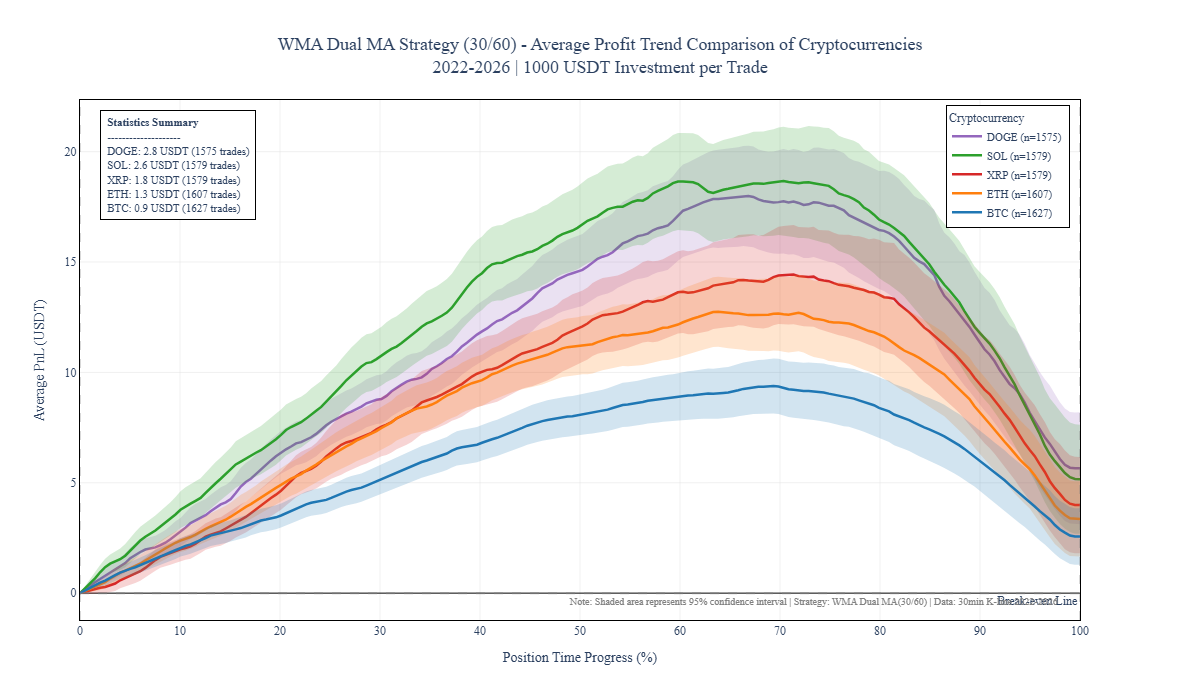
\includegraphics[width=0.85\textwidth]{figs/average_profit_trend.png}
    \caption{Average Profit Pathss Across Cryptocurrencies}
    \label{fig:average_profit_trend}
\end{figure}

Trend-following strategies are able to capture positive profit opportunities in most trades 
($MFE > 0$), indicating their effectiveness in trend identification. However, only about 30\% 
of trades are able to close with positive returns, suggesting that a large amount of unrealized 
profits is not effectively locked in. The profit path analysis shows that trades generally 
experience a dynamic process of ``profit formation--profit drawdown.'' Therefore, it can be 
concluded that unrealized profit drawdown risk is a systematic and prevalent phenomenon in 
trend-following strategies. This finding fundamentally explains the contradiction in 
trend-following strategies between ``high potential profits and low realized profits,'' and 
indicates that the exit problem is essentially a decision problem of ``profit protection'' 
rather than ``profit acquisition.'' This conclusion provides a direct theoretical motivation 
for the subsequent proposal of an early-closing decision method based on sequence learning.

\section{Methodology}
\label{sec:methodology}

\subsection{Framework Overview}

This paper proposes a hybrid decision-making framework that combines the signal identification 
capability of traditional trend-following strategies with the nonlinear risk-control capability 
of deep learning models. The framework consists of three key components: baseline strategy 
layer, LSTM decision layer, and exit execution mechanism. The baseline strategy layer uses 
weighted moving average (WMA) crossover signals as the logical starting point, and is 
responsible for capturing market trends and generating initial trading signals. The LSTM 
decision layer serves as an intelligent risk-management module embedded on top of the baseline 
strategy. By monitoring real-time market-state features and position-context information, it 
dynamically evaluates the risk of unrealized profit drawdown.

The core operating logic of the system is a two-layer collaborative mechanism. When the 
baseline strategy layer triggers an entry signal according to the moving-average crossover rule, 
the system enters the holding state. At this point, the LSTM decision layer is activated 
simultaneously. Through nonlinear mapping of the input feature sequence, it outputs in real 
time the conditional probability of whether an early closing operation should be executed at 
the current time. If the predicted probability exceeds a preset decision threshold, the system 
will execute an exit operation before the traditional trend-reversal signal appears, so as to 
lock in profits and avoid or mitigate potential large drawdown. From a system-architecture 
perspective, this model constitutes a data-driven decision layer superimposed on the 
traditional rule-based logic, thereby significantly improving the refined management capability 
of the strategy during the holding period.

\subsection{Baseline Strategy}

To ensure the sensitivity and representativeness of the empirical analysis, this paper selects 
a weighted moving average (WMA) dual moving-average system as the baseline strategy. Compared 
with a simple moving average (SMA), WMA assigns greater weights to more recent price 
observations, enabling it to respond more quickly to price changes and to exhibit greater 
flexibility in trend identification. The strategy logic adopted in this study follows a 
standard moving-average crossover rule. In terms of entry rules, the system uses the crossover 
logic of a 30-period fast moving average and a 60-period slow moving average. When the fast 
moving average crosses above the slow moving average from below, that is, when a golden cross 
is formed, a long-entry signal is executed. Conversely, when the fast moving average crosses 
below the slow moving average from above, that is, when a death cross is formed, a short-entry 
signal is executed. In terms of traditional exit rules, the baseline mechanism used for 
comparison relies only on reverse trading signals; that is, a position is closed only when an 
opposite signal to the current position direction appears. Although this mechanism can help 
capture relatively complete trend intervals, it also faces significant unrealized profit 
drawdown risk in the later stage of a trend, which constitutes the core motivation for 
introducing the LSTM decision layer in this paper.

\subsection{Problem Formulation}

In the hybrid decision-making framework proposed in this paper, the LSTM decision layer does 
not directly undertake the task of predicting trend direction. Instead, it is defined as a 
dynamic exit decision model for the holding period. In other words, the baseline strategy layer 
has already determined the trading direction according to the WMA crossover rule, while the 
core objective of the LSTM model is to judge whether the current unrealized profit faces a 
relatively high future drawdown risk during the holding process.

Let the market feature vector at time $t$ be denoted by $\mathbf{x}_t$. For any trading sample 
that is in the holding state, the model takes the feature sequence over the past $k$ time steps 
as input:

\begin{equation}
    \mathbf{X}_{t-k:t} = \{\mathbf{x}_{t-k}, \mathbf{x}_{t-k+1}, \cdots, \mathbf{x}_{t}\}
\end{equation}

The output of the LSTM decision layer is defined as the conditional probability of executing 
an early closing operation at the current time:
\begin{equation}
    p_t = P(exit \mid \mathbf{X}_{t-k:t})
\end{equation}

This probability can be regarded as a probabilistic characterization of ``unrealized profit 
drawdown risk.'' When $p_t$ is high, it indicates that the model believes that, if the position 
continues to be held, the current unrealized profit is more likely to experience a future 
drawdown. Conversely, when $p_t$ is low, it suggests that continuing to hold the position may 
still have a higher expected value than exiting immediately.

Therefore, the problem in this paper can be viewed as a sequential binary classification 
problem: given the current and historical market-state sequence $\mathbf{x}_{t-k:t}$, the model 
learns to determine whether the position should be actively exited before the reverse signal of 
the baseline strategy appears. In this way, the LSTM layer is transformed from a traditional 
``direction prediction model'' into a ``profit protection and risk control model.''

\subsection{Feature Engineering}

To enable the LSTM decision layer to perceive both the market environment and the current 
trading state, this paper constructs an input feature system jointly composed of market 
features and position-context features, providing the informational basis required for the 
model to identify future unrealized profit drawdown risk.

\subsubsection{Market Features}

When selecting market features, this paper follows the approaches of \citet{FischerKrauss2018}, 
\citet{HuangWanZhangLu2024}, and \citet{AlKhatibEtAl2022}, and jointly considers price trends, 
return-generating ability, candlestick patterns, volatility conditions, and trading activity. 
The detailed definitions of the variables are shown in Table~\ref{tab:market_features}.

\begin{table}[htbp]
\centering
\caption{Market Features}
\label{tab:market_features}
\small
\renewcommand{\arraystretch}{1.2}
\begin{tabular}{p{0.12\textwidth}p{0.34\textwidth}p{0.43\textwidth}}
\toprule
Category & Feature & Description \\
\midrule
Trend &
\texttt{wma30\_rel}, \texttt{wma60\_rel} &
Deviation of the closing price from the moving averages \\
Trend &
\texttt{wma\_spread} &
Deviation of the 30-day moving average from the 60-day moving average \\
Trend &
\texttt{wma30\_slope}, \texttt{wma60\_slope} &
First-order differences of the moving averages \\
Return &
\texttt{log\_ret}, \texttt{oc\_ret} &
Log return and open-close ratio \\
Pattern &
\texttt{hl\_range}, \texttt{shadow\_imbalance} &
Price range and upper-lower shadow imbalance \\
Volatility &
\texttt{atr14\_ret} &
ATR(14) divided by the closing price \\
Trading Activity &
\texttt{vol\_z20}, \texttt{taker\_buy\_ratio} &
Trading volume Z-score and active buy ratio \\
\bottomrule
\end{tabular}
\end{table}

\subsubsection{Position Context Features}

In addition to market features, the key innovation of this paper lies in the introduction of 
position-context features. Traditional technical indicators usually describe the market itself, 
but cannot represent the current trading state. However, for the early take-profit problem, the 
decision implications of the same market trend may differ across different stages of the 
holding period. For example, the drawdown immediately after opening a position and the drawdown 
after a large unrealized profit are not equivalent in terms of risk implications. Therefore, 
this paper represents the position state as model input. The detailed definitions of the 
variables are shown in Table~\ref{tab:position_context_features}.

\begin{table}[htbp]
\centering
\caption{Position Context Features}
\label{tab:position_context_features}
\small
\renewcommand{\arraystretch}{1.2}
\begin{tabular}{p{0.25\textwidth}p{0.60\textwidth}}
\toprule
Feature & Description \\
\midrule
\texttt{age} & Number of bars for which the current position has been held \\
\texttt{pnl\_dir} & Unrealized profit or loss in the direction of the position \\
\texttt{mfe} & Maximum favorable excursion \\
\texttt{retrace} & Drawdown from the maximum favorable excursion \\
\texttt{dir} & Position direction, where ``+1'' denotes a long position and ``-1'' denotes a short position \\
\bottomrule
\end{tabular}
\end{table}

By introducing the above position-context information, the LSTM model no longer makes decisions 
solely based on market states, but is able to make decisions according to the dynamic profit 
and loss condition of the current trade, the holding duration, and other information. This 
allows the model to more closely approximate the risk-management logic of real trading.

\subsection{Label Construction}

To train the LSTM decision layer, this paper needs to construct a supervisory label indicating 
whether an early exit should be executed for each time point in the holding state. This paper 
adopts a value-based labeling method based on the trade-off between future returns and future 
drawdowns, so that the labels can more closely reflect unrealized profit drawdown risk.

For a trade generated by the baseline strategy, let its entry time be $t_0$ and the original 
exit time of the baseline strategy be $T$. At any holding time $t$, if the position is held 
until the exit point given by the baseline strategy, the future incremental return that may 
still be obtained relative to the current time is defined as:

\begin{equation}
    future\_gain_t = pnl_T - pnl_t
\end{equation}

where $pnl_t$ denotes the unrealized profit adjusted by the current position direction, and 
$pnl_T$ denotes the profit when the baseline strategy eventually exits.

At the same time, if the position continues to be held from the current time, the price may 
experience adverse fluctuations along the future path. This paper defines the future adverse 
drawdown as $future\_drawdown_t$, which is used to measure the maximum adverse price movement 
that the trade may encounter between the current time and the baseline exit time. Based on 
this, this paper constructs the value evaluation function:

\begin{equation}
    value\_score_t = future\_gain_t - \lambda \cdot future\_drawdown_t
\end{equation}

where $\lambda$ is the risk-penalty coefficient, used to reflect investors' aversion to risk. 
When $\lambda$ is larger, the label construction process places greater emphasis on drawdown 
risk; conversely, it places more emphasis on the future returns that may be obtained by 
continuing to hold the position.

This paper uses the value score as a proxy indicator for unrealized profit drawdown risk. If 
$value\_score_t < 0$, it indicates that the potential return from continuing to hold the 
position from the current time is insufficient to compensate for the adverse drawdown that may 
occur in the future. In this case, the sample should be labeled as an early exit:

\begin{equation}
    y_t =
    \begin{cases}
    1, & \text{if } value\_score_t < 0 \\
    0, & \text{if } value\_score_t \geq 0
    \end{cases}
\end{equation}

where $y_t = 1$ indicates that an early closing operation should be executed at the current 
time, while $y_t = 0$ indicates that the position should continue to be held. In this way, the 
model's learning objective is no longer to predict the price direction, but to identify whether 
the current position is exposed to relatively high future drawdown risk.

To prevent the model from being disturbed by noise in the early stage after opening a position, 
this paper sets a minimum holding-period constraint. A sample is included in the label 
construction process only when the holding time of the trade exceeds 90 minutes and the current 
unrealized profit exceeds 0.5\%. This treatment ensures that the LSTM decision layer mainly 
serves the exit management after an unrealized profit has already emerged, rather than 
interfering with the initial entry logic of the baseline strategy.

\subsection{LSTM Model}

This paper adopts a Long Short-Term Memory (LSTM) network as the early-exit decision model. 
LSTM is suitable for capturing dynamic dependence in financial time series and can, to a 
certain extent, capture the nonlinear relationship between trend evolution and position-state 
changes.

The model input is a fixed-length historical feature matrix:

\begin{equation}
    \mathbf{X}_{t-63:t} \in \mathbb{R}^{64 \times 17}
\end{equation}

where 64 denotes the length of the time window, and 17 denotes the feature dimension contained 
in each time step.

The LSTM model recursively encodes the input sequence and uses the hidden state of the last 
time step as a comprehensive representation of the current holding state. The hidden state is 
then mapped into a one-dimensional output through a fully connected layer and converted into a 
probability form through the Sigmoid function:

\begin{equation}
    p_t = \sigma(\mathbf{w}\mathbf{h}_t + b)
\end{equation}

where $\mathbf{h}_t$ denotes the hidden state of the LSTM at the current time, $\mathbf{w}$ and 
$b$ denote the weight and bias of the fully connected layer, respectively, and $\sigma(\cdot)$ 
denotes the Sigmoid activation function. The final output is interpreted as the probability of 
early exit at the current time, namely:

\begin{equation}
    p_t = P(y_t = 1 \mid \mathbf{X}_{t-63:t})
\end{equation}

When $p_t$ is close to 1, it indicates that the model believes the future unrealized profit 
drawdown risk is relatively high and that the current position should be closed early. When 
$p_t$ is close to 0, it indicates that continuing to hold the position is more reasonable.

\subsection{Decision Rule}

In the backtesting stage, the LSTM decision layer operates as an additional exit module on top 
of the baseline strategy. The baseline strategy still generates trading directions and initial 
entry signals, while the LSTM model participates in decision-making only when an existing 
position is being held.

Specifically, when the system executes a WMA crossover rule based on the baseline strategy and 
establishes a position, for each new candlestick, the market features and position-context 
features are updated, and the feature sequence of the most recent 64 time steps is input into 
the LSTM model to obtain the early-exit probability $p_t$.

The exit rule in this paper can be expressed as:

\begin{equation}
    Exit_t =
    \begin{cases}
    1, & p_t > \theta \\
    -1, & \text{opposite WMA crossover occurs} \\
    0, & \text{else}
    \end{cases}
\end{equation}

where $\theta$ is the decision threshold for early exit, determined through grid search, and 
the results are shown in Table~\ref{tab:decision_threshold}. When $p_t > \theta$, it indicates 
that the model judges the current position to face a relatively high future unrealized profit 
drawdown risk, and therefore the system will actively close the position before the reverse 
crossover signal of the baseline strategy appears. If the LSTM does not trigger an early exit, 
the trade continues to be managed according to the original moving-average reverse crossover 
rule.

\begin{table}[htbp]
\centering
\caption{Backtesting Results under Different LSTM Decision Thresholds}
\label{tab:decision_threshold}
\small
\setlength{\tabcolsep}{4pt}
\renewcommand{\arraystretch}{1.15}
\resizebox{\textwidth}{!}{
\begin{tabular}{lrrrrrrr}
\toprule
\makecell{Threshold\\$\theta$} &
\makecell{Number of\\LSTM Exits} &
\makecell{LSTM Exit\\Ratio (\%)} &
\makecell{Cumulative\\Return (\%)} &
\makecell{Win\\Rate (\%)} &
\makecell{Sharpe\\Ratio} &
\makecell{Average Holding\\Bars} &
\makecell{Maximum\\Drawdown} \\
\midrule
Baseline & 0   & 0.0  & +1.2807 & 36.7 & 2.252 & 48.9 & 0.2782 \\
0.30     & 142 & 68.6 & +0.4161 & 68.6 & 3.723 & 11.2 & 0.1045 \\
0.40     & 141 & 68.1 & +0.4511 & 68.1 & 3.842 & 11.6 & 0.1390 \\
0.50     & 121 & 58.5 & +0.8222 & 64.3 & 3.960 & 18.6 & 0.1336 \\
0.55     & 58  & 28.0 & +0.9526 & 51.2 & 2.602 & 34.2 & 0.1351 \\
$\geq 0.60$ & 0 & 0.0 & +1.2807 & 36.7 & 2.252 & 48.9 & 0.2782 \\
\bottomrule
\end{tabular}
}
\end{table}

Through the above decision rule, this paper forms a two-layer exit mechanism: the baseline 
strategy provides trend-reversal exits, while the LSTM layer provides risk-warning-based early 
exits. The former ensures that the strategy still follows trend-following trading logic, while 
the latter improves the responsiveness to unrealized profit drawdown risk during the holding 
period. This mechanism enables the strategy to no longer passively wait for the moving-average 
reverse crossover, but instead to lock in profits in advance when drawdown risk rises, thereby 
improving strategy performance.

\section{Experimental Design}

\subsection{Dataset}

To objectively evaluate the generalization ability of the LSTM-based early-closing decision 
framework in dynamic market environments, this study selects the cryptocurrency market as the 
empirical setting. The cryptocurrency market features 24/7 continuous trading, high volatility, 
and pronounced trend persistence, making it an ideal setting for testing whether the enhanced 
strategy can effectively improve the traditional trend-following model.

This study selects five mainstream cryptocurrency trading pairs as the 
experimental assets: BTC/USDT, ETH/USDT, SOL/USDT, XRP/USDT, and DOGE/USDT. These assets cover 
different market capitalizations, liquidity characteristics, and price fluctuation patterns, 
thereby allowing the robustness of the model across assets to be evaluated.

The raw market data used in the experiment range from January 1, 2022 to March 12, 2026. This 
interval fully covers multiple bull-bear cycles in the market, enabling the model to be tested 
across different market regimes, including trend continuation, range-bound fluctuation, and 
sharp drawdown. In this paper, 30-minute candlestick data are used for modeling. This time 
granularity ensures the reliability of trend signals while providing sufficient sequence depth 
for the LSTM model, so as to capture the dynamic evolution of micro risk structures during the 
holding period.

This study strictly follows the chronological order principle for predictive samples, and 
divides the dataset into the training set, validation set, and testing set, with proportions of 
approximately 70\%, 15\%, and 15\%, respectively. The specific sample sizes and corresponding 
time intervals are shown in Table~\ref{tab:dataset_split}.

\begin{table}[htbp]
\centering
\caption{Dataset Split}
\label{tab:dataset_split}
\small
\setlength{\tabcolsep}{4pt}
\renewcommand{\arraystretch}{1.2}
\begin{tabular}{p{0.15\textwidth}p{0.12\textwidth}p{0.14\textwidth}p{0.18\textwidth}p{0.32\textwidth}}
\toprule
Stage & Proportion & Sample Size & Time Interval & Research Function \\
\midrule
\makecell{Training\\Set} &
70\% &
29,250 &
\makecell{2022/01/02--\\2025/01/06} &
Model parameter learning and weight optimization \\

\makecell{Validation\\Set} &
15\% &
6,268 &
\makecell{2025/01/06--\\2025/08/05} &
Hyperparameter tuning and overfitting prevention \\

\makecell{Testing\\Set} &
15\% &
6,269 &
\makecell{2025/08/05--\\2026/03/11} &
Out-of-sample evaluation and robustness test \\
\bottomrule
\end{tabular}
\end{table}

\subsection{Data Cleaning}

This paper first conducts basic cleaning on the raw candlestick data, including uniformly 
parsing the time field into UTC time format, converting fields such as prices and trading 
volume into numerical types, and sorting the data in chronological order. Subsequently, 
anomaly auditing is performed on the raw sequence to identify missing candlesticks, 
zero-volume candlesticks, and extreme fluctuation samples, with corresponding flags 
constructed for each type of anomaly. Since the LSTM model adopts a fixed-length historical 
window for modeling, this paper further constructs a context-contamination flag using a 
rolling-window method, and removes samples whose historical windows contain bad data from the 
training dataset.

\subsection{Comparison Methods}

To examine whether the proposed Long Short-Term Memory (LSTM)-based early-closing decision 
framework can further improve performance on top of traditional trading strategies, this paper 
sets up several representative benchmark methods for comparative experiments. Specifically, 
the proposed LSTM early-closing strategy is compared with the WMA baseline strategy, the fixed 
take-profit strategy, and the trailing take-profit strategy, in order to evaluate its 
effectiveness in enhancing returns, controlling drawdowns, and improving risk-adjusted returns.

First, the WMA baseline strategy serves as the fundamental trend-following strategy in this 
paper, and is used to characterize the original strategy performance without introducing any 
additional early-closing mechanism. This method mainly relies on 30-day and 60-day weighted 
moving average signals for opening and closing positions, thereby providing a basic reference 
for evaluating whether subsequent exit-optimization methods are effective.

Second, the fixed take-profit strategy is a simple and commonly used rule-based exit method. 
It triggers position closing once the holding return reaches a fixed threshold, which is set 
to 10\% in this paper. The advantage of this method lies in its clear rules and stable 
execution. However, its limitation is that it cannot adjust dynamically according to market 
conditions, which may lead to premature profit taking or failure to avoid profit drawdowns in 
a timely manner.

Third, the trailing take-profit strategy is used to represent a more dynamic traditional 
risk-control method. When the holding return reaches a preset threshold, which is set to 3\% 
in this paper, the strategy enters a take-profit monitoring state. Thereafter, if the current 
holding return falls by more than a preset threshold from the highest unrealized profit level 
reached during the holding period, which is set to 10\% in this paper, the position is closed. 
Compared with the fixed take-profit strategy, the trailing take-profit strategy can preserve 
the potential for further gains during trending markets to some extent while controlling the 
drawdown of unrealized profits. Therefore, it serves as an important benchmark for testing 
whether the proposed method has stronger dynamic risk-identification capability.

In terms of experimental design, this paper applies the above strategies uniformly to 
multiple mainstream cryptocurrency trading pairs, including BTC/USDT, ETH/USDT, SOL/USDT, 
XRP/USDT, and DOGE/USDT, and compares their performance across different assets. Through 
cross-asset experiments, the robustness of the proposed method can be further examined.

\subsection{Evaluation Metrics}

To comprehensively evaluate the performance of different strategies and models in the 
early-closing task, this paper constructs an evaluation metric system from five dimensions: 
profitability, risk-adjusted return, drawdown control, trading stability, and holding 
efficiency. Specifically, the metrics include cumulative return, Sharpe ratio, maximum 
drawdown, win rate, and average holding time.

First, cumulative return is used to measure the overall profitability of the strategy during 
the testing period. This metric reflects the growth of the initial capital after the complete 
backtesting period and is the most direct indicator for evaluating strategy return 
performance. It is calculated as follows:

\begin{equation}
    Ret = \frac{V_T - V_0}{V_0}
\end{equation}

where $V_0$ denotes the initial capital size, and $V_T$ denotes the capital size at the end 
of the backtesting period. A higher cumulative return indicates stronger overall profitability 
during the out-of-sample testing period.

Second, the Sharpe ratio is used to measure the excess return obtained by the strategy per 
unit of risk taken. Compared with a simple return metric, the Sharpe ratio further considers 
return volatility, and therefore can better reflect the risk-adjusted return performance of 
the strategy. It is calculated as follows:

\begin{equation}
    SharpeR = \frac{R_p - R_f}{\sigma_p}
\end{equation}

where $R_p$ denotes the strategy return, $R_f$ denotes the risk-free rate, and $\sigma_p$ 
denotes the standard deviation of strategy returns. In high-frequency or short-period 
cryptocurrency backtesting, since each holding period is relatively short, the risk-free rate 
can be approximately set to zero in this paper. A higher Sharpe ratio indicates that the 
strategy can obtain higher returns under the same level of risk.

Third, maximum drawdown is used to measure the maximum capital loss that the strategy may 
suffer during the backtesting period, and is an important indicator for evaluating the 
risk-control capability of the strategy. It is calculated as follows:

\begin{equation}
    MDD = \max_{t \in [0,T]} \frac{V^{peak}_t - V_t}{V^{peak}_t}
\end{equation}

where $V_t$ denotes the net asset value at time $t$, and $V^{peak}_t$ denotes the historical 
highest net asset value up to time $t$. A smaller maximum drawdown indicates stronger 
capital-protection capability under adverse market fluctuations. For an early-closing strategy, if the model can identify profit drawdown risk in a timely manner, it should reduce the maximum drawdown to some extent.

Fourth, the win rate is used to measure the stability of trading outcomes, and represents the 
proportion of profitable trades among all trades. It is calculated as follows:

\begin{equation}
    WinRate = \frac{N_{win}}{N_{total}}
\end{equation}

where $N_{win}$ denotes the number of profitable trades, and $N_{total}$ denotes the total 
number of trades. A higher win rate indicates that the strategy generates profitable trades 
more frequently. However, the win rate alone cannot represent the overall quality of a 
strategy, because a high-win-rate strategy may still produce poor overall returns due to a 
small number of large losses. Therefore, this paper analyzes it jointly with cumulative return, 
Sharpe ratio, and maximum drawdown.

Finally, average holding time is used to measure the average duration from opening to closing 
a position, reflecting the impact of different closing mechanisms on the holding period. It is 
calculated as follows:

\begin{equation}
    AvgHT = \frac{1}{N} \sum_{i=1}^{N} \left(t^{exit}_i - t^{entry}_i\right)
\end{equation}

where $t^{entry}_i$ and $t^{exit}_i$ denote the opening time and closing time of the $i$-th 
trade, respectively, and $N$ denotes the total number of trades. Average holding time can 
reflect whether a strategy tends to exit too early or hold positions for a long time. For the 
LSTM-based early-closing framework proposed in this paper, this metric helps determine whether 
the model can avoid subsequent drawdown risk in a timely manner while preserving the profit 
potential of trend-following trades.

\section{Results}
\section{Discussion}
\section{Robustness Checks}
\section{Conclusion}
\section{Future Work}



























\newpage

% =========================
% References
% =========================
\bibliographystyle{apalike}
\bibliography{references}

\newpage

% =========================
% Appendix
% =========================
\appendix

\section{Additional Tables}

\begin{table}[H]
\centering
\caption{Variable Definitions}
\label{tab:variables}
\begin{tabular}{ll}
\toprule
Variable & Definition \\
\midrule
$Flow_t^{5d}$ & Five-day change in stablecoin market capitalization \\
$\Delta \ln Flat_t$ & Growth rate of fiat-reserve-backed stablecoin market capitalization \\
$\Delta \ln Coll_t$ & Growth rate of collateralized stablecoin market capitalization \\
$\Delta y_t$ & Change in Treasury yield \\
$X_t$ & Vector of control variables \\
\bottomrule
\end{tabular}
\end{table}

\section{Additional Figures}

Additional figures can be placed here.

\end{document}